\chapter{Verification and Validation of the Fluid-Structure Interaction Implementation}\label{chap:VV}
When investigating a real world problem with a numerical model, the general approach is to: describe the problem with a mathematical model, discretize and implement the model on a computer, and finally simulate the implemented model to gain insight into the real world problem.

A question then immediately arises, computer models have been known to be incorrect in the past \cite{oberkampf2008verification}, how can we trust the insight gained from numerical simulation? 
To answer this question we need to adress another question, are the equations implemented correct? If so, is the mathematical description of the problem adequately defined? 
Without answering these questions, being confident that your solutions are correct is difficult \cite{oberkampf2008verification}. The process of generating evidence that computed solutions meets certain requirements to fulfill an intended purpose, in the context of scientific computing, is known as Verification and Validation. The goal of this section will hence be to verify and validate the different numerical schemes outlined in the two previous chapters.  \\

The chapter starts with the process of Verification, where the fluid and structure numerical schemes will be verified separately. Then use a well known benchmark to validate the fluid, structure, and FSI models, separately. \newline

\section{Verification}
Verification, in the context of scientific computing, is the process of determining wether or not the implementation of numerical algorithms in computer code, is correct \cite{Oberkampf2010}.
Mapping a mathematical model to a computational model there will always be introduced an error, often referred to as truncation error. Verification helps us identify, quantify, and reduce the errors, assuring that there are no coding mistakes which effects the truncation error. Verification does not address wether or not the computed solutions are in alignment with physics in the real world. It only tells us that our model is computed correctly or not. \newline

In Verification there are multiple classes of test that can be performed, one of which is \textit{order of convergence tests}. Order of convergence are based on the behavior of the error between a known exact solution and a computed solution \cite{Roache2002}. The most rigorous of the order of convergence test is the \textit{Method of Manufactured Solution} (MMS) \cite{Oberkampf2010}. When performing a MMS test, rather than looking for an exact solution, we manufacture one. The idea is to create a solution \textit{a priori}, and use this solution to generate an analytical source term for the governing PDEs and then compute the PDE with the source term to produce a solution. The manufactured solution does not need to have a physically realistic relation, since the solution is only testing the mathematics. \newline

When manufacturing a solution in MMS tests there are a number of criteria that needs to be met for a solution to be sufficient. The manufactured solutions should be chosen to be non-trivial and analytic \cite{Oberkampf2010, Roache2002}. The solutions should be manufactured such that all terms of the equation are of the same order of magnitude. For this reason trigonometric and exponential functions can be a smart choice, since they are smooth and infinitely differentiable. In short, a good manufactured solution is one that is complex enough so that it rigorously tests each part of the equations.\newline 

The procedure of MMS is as follows \cite{Oberkampf2010}:
\begin{itemize}
\item We define a mathematical model on the form $ L(\bold{u}) = 0$, where $L(\bold{u})$ is a differential operator and $u$ is a dependent variable.
\item Define the analytical form of the manufactured solution $\hat{\bold{u}}$
\item Use the model $L(u)$ with $\hat{\bold{u}}$ inserted to obtain an analytical source term $ f = L(\hat{\bold{u}}) $
\item Initial and boundary conditions are enforced from $\hat{\bold{u}}$
\item Find the numerical solution of the problem with the given source term, $L(\bold{u}) = f $
\end{itemize}

If we let $\bold{u}$ be the numerical solution and $\hat{\bold{u}}$ be the exact solution, $|| . ||$ be the $L^2$ norm, the error can be computed as:
\begin{equation}
E = || \bold{u} - \hat{\bold{u}} ||
\end{equation}
When we decrease the node spacing ($ \Delta x $) or decrease time step size ($\Delta t$), we expect the solution to convergence towards a given solution and hence the error becomes smaller. If we assume uniform node spacing in all spatial directions: 
\begin{equation}
\label{eq:Error}
 E = C_1 \Delta x^k+ C_2 \Delta t^l 
\end{equation}
where $C_1$ and $C_2$ are constants, $ k = m+1 $ and m is the polynomial degree of the spatial elements. The error is hence dependent on the node spacing and the time step.
In order to compute the convergence k  based on the error, we first have to let the term with $C_2\Delta t^l$ be negligible compared to $C_1\Delta x^2$. 
Let $E_{n+1}$ and $E_{n}$ be the computed errors of a solution with fine and coarse node spacing respectively.
Using equation \eqref{eq:Error} we can find $k$ by:
\begin{align}
\frac{E_{n+1}}{E_n} = \big( \frac{\Delta x_{n+1}}{\Delta x_n} \big)^k \\
k = \frac{log( \frac{E_{n+1}}{E_n}) }{ log(\frac{\Delta x_{n+1}}{\Delta x_n})}
\end{align}
After refining the mesh while keeping $\Delta t $ fixed and sufficiently small,
$k$ can be compared to the theoretical order of convergence for each given problem. If the k that we have found matches the theoretical order of convergence, with small margin of error, there are no coding mistakes present which effects the order of convergence, and thus the accuracy of the numerical scheme. \newline


\section{Structure MMS}
To do MMS of the solid I use the solid equation and make a sourceterm $f_s$:
$$\rho_s \frac{\partial u}{\partial t} - \nabla \cdot ( P ) = f_s $$
The solid variational formulation is written as:
\begin{align}
\big(\rho_s \frac{\partial u}{\partial t},\phi \big)_{\mathcal{\hat{S}}} + \big(P, \nabla \phi \big)_{\mathcal{\hat{S}}} &=f_s \\
\big( u- \frac{\partial d}{\partial t} ,\psi \big)_{\mathcal{\hat{S}}} &= 0 
\end{align}
These equations are solved together and we solve for $d$ and $u$. The functions u and d will be computed to match the source term. In the tables below we investigate convergence in space and time. \newline

Even though we have two equations we do not make a source for the second. This is because the solutions are made to uphold criteria of $u = \frac{\partial d}{\partial t}$:
\begin{align*}
d =& ( cos(y)sin(t) , cos(x)sin(t) )\\
u =& ( cos(y)cos(t), cos(x)cos(t) )
\end{align*}
To meet the requirements of MMS such as smoothness and complexity, i chose functions with sine and cosine. The derivatives does not become zero and we have time and space dependencies. 
\newline

I start with checking order of convergence in space. Setting m = 1, the expected order of convergence will 2. 

\begin{table}[H]
\centering
\caption{Structure Method of Manufactured of Solution in space in m = 1}
\label{my-label}
\begin{tabular}{|l|l|l|l|l|l|l|}
\hline
\textbf{N}  & $\Delta t$  & \textbf{m} & $E_u \times 10^{-3}$ & $\bold{k_u}$    & $E_d \times 10^{-8}$ & $\bold{k_d}$    \\ \hline
\textbf{4}  & $1\times10^{-6}$ & \textbf{1} & 6.88                 & \textbf{}         & 3.78                 & \textbf{}         \\ \hline
\textbf{8}  & $1\times10^{-6}$ & \textbf{1} & 1.72                 & \textbf{2.000212} & 0.94                 & \textbf{2.000212} \\ \hline
\textbf{16} & $1\times10^{-6}$ & \textbf{1} & 0.43                 & \textbf{2.000051} & 0.23                 & \textbf{2.000051} \\ \hline
\textbf{32} & $1\times10^{-6}$ & \textbf{1} & 0.10                 & \textbf{2.000012} & 0.05                 & \textbf{2.000012} \\ \hline
\textbf{64} & $1\times10^{-6}$ & \textbf{1} & 0.026                & \textbf{2.000003} & 0.0014               & \textbf{2.000003} \\ \hline
\end{tabular}
\end{table}

Up next I set m=2 changing the expected order of convergence to 2:

\begin{table}[H]
\centering
\caption{Structure Method of Manufactured of Solution in space in m = 2}
\label{my-label}
\begin{tabular}{|l|l|l|l|l|l|l|}
\hline
\textbf{N} & $\Delta t$ & \textbf{m} & $E_u [\times 10^-5]$ & $\bold{k_u}$ & $E_d [\times 10^{-10}]$ & $\bold{k_d}$ \\ \hline
\textbf{4} & $1\times10^{-6}$ & \textbf{2} & 6.60 & \textbf{-} & 3.63 & \textbf{-} \\ \hline
\textbf{8} & $1\times10^{-6}$ & \textbf{2} & 0.82 & \textbf{2.99458} & 0.45 & \textbf{2.99458} \\ \hline
\textbf{16} & $1\times10^{-6}$ & \textbf{2} & 0.10 & \textbf{2.99865} & 0.057 & \textbf{2.99865} \\ \hline
\textbf{32} & $1\times10^{-6}$ & \textbf{2} & 0.012 & \textbf{2.99966} & 0.0071 & \textbf{2.99966} \\ \hline
\textbf{64} & $1\times10^{-6}$ & \textbf{2} & 0.00161 & \textbf{2.99991} & 0.00089 & \textbf{2.99991} \\ \hline
\end{tabular}
\end{table}

Lastly I check convergence in time. Here i set N = 64 and the timestep is halved for each computation.

\begin{table}[H]
\centering
\caption{Structure Method of Manufactured of Solution in time}
\label{my-label}
\begin{tabular}{|l|l|l|l|l|l|}
\hline
N & $\bold{\Delta t}$ & $E_u [\times10^{-6}]$ & $\bold{k_u}$ & $E_u [\times10^{-8}]$ & $\bold{k_d}$ \\ \hline
64 & \textbf{0.0008} & 2.40 & \textbf{-} & 1.76 & \textbf{-} \\ \hline
64 & \textbf{0.0004} & 1.20 & \textbf{0.995} & 0.86 & \textbf{1.0233} \\ \hline
64 & \textbf{0.0002} & 0.59 & \textbf{1.026} & 0.41 & \textbf{1.0676} \\ \hline
64 & \textbf{0.0001} & 0.29 & \textbf{1.011} & 0.20 & \textbf{1.0338} \\ \hline
64 & \textbf{0.00005} & 0.14 & \textbf{0.998} & 0.10 & \textbf{1.0138} \\ \hline
\end{tabular}
\end{table}


\section{MMS on FSI ALE}
In this section we use the method of manufactured solutions to verify the FSI ALE monolithic solver. We start by prescribing a motion to $ d$ and $w$ and give a solution to $u$ and $p$. We set $u = w$ to start with:
\begin{align*}
d =& ( cos(y)sin(t) , cos(x)sin(t) )\\
u = w=& ( cos(y)cos(t), cos(x)cos(t) ) \\
p =& cos(x)cos(t)
\end{align*}
We make the solutions to uphold the criterias : $ \nabla \cdot u =0  $ and $ \frac{\partial d}{\partial t} = w  $ \\

To test the mapping we make the source term $f$ without mappings:
$$ \rho_f \frac{\partial u}{\partial t}  +  \nabla u (u-\frac{\partial d}{\partial t})  -  \nabla \cdot \sigma_f  = f $$
Then we use this f and map it to the reference configuration and compute:
$$ \rho_f J \frac{\partial u}{\partial t} + (\nabla u)F^{-1}(u-\frac{\partial d}{\partial t})  + \nabla \cdot( J \hat{\sigma_f} F^{-T}) = J f$$
The computations are done on a unitsquare domain and the computations ran with 10 timesteps and the error was calculated for each time step and then the mean of all the errors was taken and used to calculate the convergence rates.
\begin{table}[h!]
\centering
\caption{MMS ALE FSI u=w}
\label{my-label}
\begin{tabular}{|l|l|l|l|l|l|l|}
\hline
N & $\Delta t$ & m & $E_u$ & $k_u$ & $E_p$ & $k_p$ \\ \hline
64 & 0.1 & 2 & 0.0140496662424 & - & 4.78779559903 & - \\ \hline
64 & 0.05 & 2 & 0.00697215098985 & 1.01086014072 & 2.38002096658 & 1.00838727906 \\ \hline
64 & 0.025 & 2 & 0.00341287458821 & 1.03061641184 & 1.18981484439 & 1.00023719999 \\ \hline
64 & 0.0125 & 2 & 0.00164214907307 & 1.05540230133 & 0.595733372533 & 0.99799839775 \\ \hline
2 & $10x^{-6}$ & 2 & 0.000520027806571 & - & 0.0194221106771 & - \\ \hline
4 & $10x^{-6}$ & 2 & 6.60205272446e-05 & 2.97760220293 & 0.00480815191132 & 2.01414560945 \\ \hline
8 & $10x^{-6}$ & 2 & 8.28184559099e-06 & 2.99489045 & 0.00118568799584 & 2.0197580517 \\ \hline
16 & $10x^{-6}$ & 2 & 1.0417232845e-06 & 2.99098020306 & 0.000281586546806 & 2.0740741124 \\ \hline
\end{tabular}
\end{table}





\newpage















\section{Validation}
After the code has been verified, we move on to Validation which is the process of determining if a model gives an accurate representation of real world physics within the bounds of the intended use \cite{oberkampf2008verification}. Depending on the quantities of interest and the problem at hand the computational model has to be validated. However, when solving a multiphysics problem, good benchmarks and trustworthy experimental data might be difficult to produce \cite{Macal2005}. Therefore we will here validate the solver, \textsl{brick by brick}, starting with simple testing of each part of the model and building more complexity and eventually testing the entire model.\newline

\begin{comment}
Three aspects have been identified in the process of validating a computational model \cite{oberkampf2008verification}. These are: quantifying the accuracy of the model by comparing responses with experimental responses, interpolation of the model to conditions corresponding to the intended use and determining the accuracy of the model for the conditions under which its meant to be used. \newline
\end{comment}

In the benchmarks used for validation, there are 9 different tests. For each test a refinement with respect to temporal an spatial resolution is performed. However, one major draw back is that the results of the benchmark were known a priori. It is easier to mold the model to the data we already have, and as Oberkampf and Trucano in \cite{oberkampf2008verification} puts it \say{Knowing the \say{correct} answer beforehand is extremely seductive, even to a saint}. Knowing the limitations of our tests will therefore strengthen our confidence in the model. The process of verifying and validating, if one does not clearly know the bounds of sufficient accuracy, is an endless process \cite{oberkampf2008verification}. 


\section*{Fluid-Structure Interaction between an elastic object and laminar incompressible flow}
The goal of this benchmark is to test the fluid and solid solver first separately and then together as a full FSI problem \cite{Hron2006a}. This benchmark is based on the older benchmark \" flow around cylinder\" with fluid considered incompressible and in the laminar regime, and the structure deformations are significant. The problem is setup with the solid submerged in the fluid, so that oscillations in the fluid deform the structure. We will measure the drag and lift around the circle and bar, and measure structural displacement at a given point. 

\subsection*{Problem Defintion}
\subsubsection*{Domain}
\begin{center}
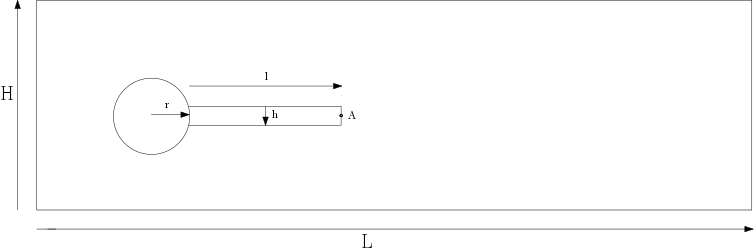
\includegraphics[scale=0.4]{./Verification_Validation/Hron_Turek/Domain_drawing.png}
\end{center}
The computational domain consists of a circle with an elastic bar behind the circle. The circle is positioned at (0.2, 0.2) making it 0.05 of center from bottom to top, this is done to induce oscillations to an otherwise laminar flow. 
This gives a force to the elastic bar. The parameters of the domain are:\\
L = 2.5, H = 0.41, l = 0.35, h = 0.02, A = (0.2,0.6) \\

\subsubsection*{Boundary conditions}
The fluid velocity has a parabolic profile on the inlet that changes over time:\\

\begin{align*}
u(0,y) &= 1.5u_0 \frac{y(H-y)}{(\frac{H}{2})^2}  \\
u(0,y,t) &= u(0,y)\frac{1-cos(\frac{\pi}{2}t)}{2} \text{  for  } t<2.0 \\
u(0,y,t) &= u(0,y) \text{  for  } t \leq 2.0
\end{align*}

We set no slip on the "floor" and "ceiling" so to speak.\\
$$ u(x,y,t) = 0 \text{  on  }  $$
On the fluid solid interface the boundary conditions are set to:
$$  \sigma_f n_f = \sigma_s n_s \hspace{4mm} on  \hspace{2mm}\Gamma^0 (interface)   $$
In our variational form we leave this out and so implying that they are equal.

\subsubsection*{Quantities for comparison}
When the fluid moves around the circle and bar it exerts a force. These are split into drag and lift and calculated as follows:
$$ (F_d, F_L) = \int_S \sigma_f n dS $$ 
where S is the part of the circle and bar in contact with the fluid. \\
We set a point A on the right side of the bar. This point is used to track the deformation in CSM and FSI tests. \\
In each test the numbers with ref are the values taken from the benchmark paper \cite{Hron2006a}
We integrate the mapped fluid stress tensor over the bar and circle and appended to lists: 
\begin{lstlisting}[language=Python]
Dr = -assemble((sigma_f_new(v,p,d,mu_f)*n)[0]*ds(6))
Li = -assemble((sigma_f_new(v,p,d,mu_f)*n)[1]*ds(6))
Dr += -assemble((sigma_f_new(v("-"),p("-"),d("-"),mu_f)*n("-"))[0]*dS(5))
Li += -assemble((sigma_f_new(v("-"),p("-"),d("-"),mu_f)*n("-"))[1]*dS(5))
Drag_list.append(Dr)
Lift_list.append(Li)
\end{lstlisting}
The deformation is calculated on the point A, and also added to lists:
\begin{lstlisting}[language=Python]
dsx = d(coord)[0]
dsy = d(coord)[1]
dis_x.append(dsx)
dis_y.append(dsy)
\end{lstlisting}
\subsection{Results}
\subsubsection*{CFD test}
The first two CFD tests are run with Reynolds number 20 and 100 giving steady drag and lift around the circle. CFD 3 has a Reynolds number 200 which will induce oscillations behind the circle, giving fluctuations in the drag and lift.
The CFD tests were run using the the bar as rigid object, that is the domain calculated is just the fluid domain. It is possible to also calculate with the bar and setting $\rho_s$ and $\mu_s$ to a large value. 

\begin{table}[h!]
\centering
\caption{CFD parameters}
\label{my-label}
\begin{tabular}{|l|l|l|l|}
\hline
Parameters & CFD1 & CFD2 & CFD3 \\ \hline
$\rho_f [10^3 \frac{kg}{m^3}]$ & 1 & 1 & 1 \\ \hline
$\nu_f [10^{-3} \frac{m^2}{s}]$ & 1 & 1 & 1 \\ \hline
$ U [\frac{m}{s}] $ & 0.2 & 1 & 2 \\ \hline
Re = $\frac{Ud}{\nu_f}$ & 20 & 100 & 200 \\ \hline
\end{tabular}
\end{table}

\begin{table}[h!]
\centering
\caption{CFD 1}
\label{my-label}
\begin{tabular}{|l|l|l|l|}
\hline
\textbf{elements} & \textbf{dofs} & \textbf{Drag} & \textbf{Lift} \\ \hline
6616 & 32472 & 14.2439 & 1.0869 \\ \hline
26464 & 124488 & 14.2646 & 1.11085 \\ \hline
105856 & 487152 & 14.2755 & 1.11795 \\ \hline
\textbf{ref} & \textbf{} & \textbf{14.29} & \textbf{1.119} \\ \hline
\end{tabular}
\end{table}

\begin{table}[h!]
\centering
\caption{CFD 2}
\label{my-label}
\begin{tabular}{|l|l|l|l|}
\hline
\textbf{elements} & \textbf{dofs} & \textbf{Drag} & \textbf{Lift} \\ \hline
6616 & 32472 & 135.465 & 6.27158 \\ \hline
26464 & 124488 & 136.566 & 9.82166 \\ \hline
105856 & 487152 & 136.573 & 10.4441 \\ \hline
\textbf{ref} & \textbf{} & \textbf{136.7} & \textbf{10.53} \\ \hline
\end{tabular}
\end{table}

\subsubsection*{CSM test}
The CSM test are calculated using only the bare and adding a gravity term $g$ with the same value but changing the parameters of solid.
As with the CFD test the first to CSM test cause a steady state solution, and CSM 3 is more slender causing the bar to go up and down in time. Our quantity for comparing there will be the deformation of the point $A$. In CSM 3 the energy is conserved by using a Crank-Nicholson scheme as can be seen in the plots fig7 (hvordan citer man et plot?)

\begin{table}[h!]
\centering
\caption{Parameters}
\label{my-label}
\begin{tabular}{|l|l|l|l|}
\hline
Parameters & CSM1 & CSM2 & CSM3 \\ \hline
$\rho_f[10^3 \frac{kg}{m^3}]$ & 1 & 1 & 1 \\ \hline
$\nu_f [10^{-3} \frac{m^2}{s}]$ & 1 & 1 & 1 \\ \hline
$u_0$ & 0 & 0 & 0 \\ \hline
$\rho_s[10^3 \frac{kg}{m^3}]$ & 1 & 1 & 1 \\ \hline
$\nu_s$ & 0.4 & 0.4 & 0.4 \\ \hline
$\mu_s[10^6 \frac{m^2}{s}]$ & 0.5 & 2.0 & 0.5 \\ \hline
$g $ & 2 & 2 & 2 \\ \hline
\end{tabular}
\end{table}

\begin{table}[h!]
\centering
\caption{CSM 1}
\label{my-label}
\begin{tabular}{|l|l|l|l|}
\hline
elements & dofs & ux $[10^{?3}]$ & uy $[10^{?3}]$ \\ \hline
725 & 1756 & -5.80951654915 & -59.4781430115 \\ \hline
2900 & 6408 & -6.77960453995 & -64.2130757639 \\ \hline
11600 & 24412 & -7.08597041285 & -65.635825349 \\ \hline
46400 & 95220 & -7.11626976966 & -65.7456687273 \\ \hline
ref & ref & -7.187 & -66.10 \\ \hline
\end{tabular}
\end{table}

% Please add the following required packages to your document preamble:
% \usepackage{booktabs}
\begin{table}[h!]
\centering
\caption{CSM 2}
\label{my-label}
\begin{tabular}{@{}|l|l|l|l|@{}}
\hline
Elements & Dofs & ux $[10^{-3}] $& ux $[10^{-3}] $\\ \hline
725 &  1756 & -0.375962146908 & -15.1950342598 \\ \hline
2900 & 6408 & -0.441308781709 & -16.4643196042\\ \hline
11600 & 24412 & -0.462087305294 & -16.8478689583 \\ \hline
46400 & 95220 & -0.464128022327 & -16.8782135872\\ \hline
ref & ref & -0.4690 & -16.97 \\ \hline
\end{tabular}
\end{table}

\begin{table}[h!]
\centering
\caption{CSM 3}
\label{my-label}
\begin{tabular}{|l|l|l|l|}
\hline
elements & dofs & ux $[10^3]$ & uy $[10^3]$ \\ \hline
725 & 1756 & $-11.743 \pm 11.744$ & $-57.952 \pm 58.940$ \\ \hline
2900 & 6408 & $-13.558 \pm 13.559$ & $ -61.968 \pm  63.440 $ \\ \hline
11600 & 24412 & $ -14.128 \pm 14.127$ & $-63.216 \pm 64.744 $ \\ \hline
46400 & 95220 & $ -14.182 \pm 14.181 $ & $ -63.305 \pm 64.843 $ \\ \hline
ref &  & $-14.305 \pm 14.305 $ & $-63.607 \pm 65.160 $ \\ \hline
\end{tabular}
\end{table}

\begin{figure}[h!] 
  \begin{subfigure}[b]{0.5\linewidth}
    \centering
    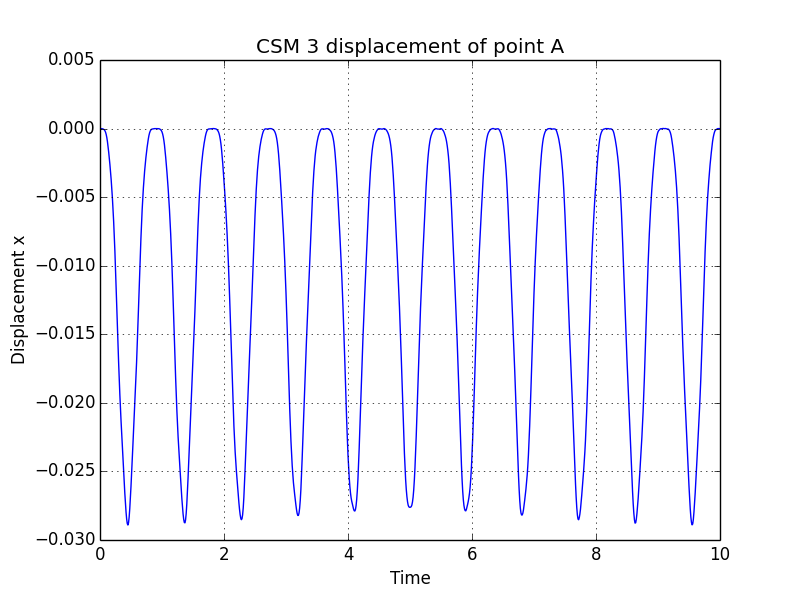
\includegraphics[width=0.75\linewidth]{./Verification_Validation//Hron_Turek/dis_x.png} 
    \caption{Displacement in x-direction} 
    \label{fig7:a} 
    \vspace{4ex}
  \end{subfigure}%% 
  \begin{subfigure}[b]{0.5\linewidth}
    \centering
    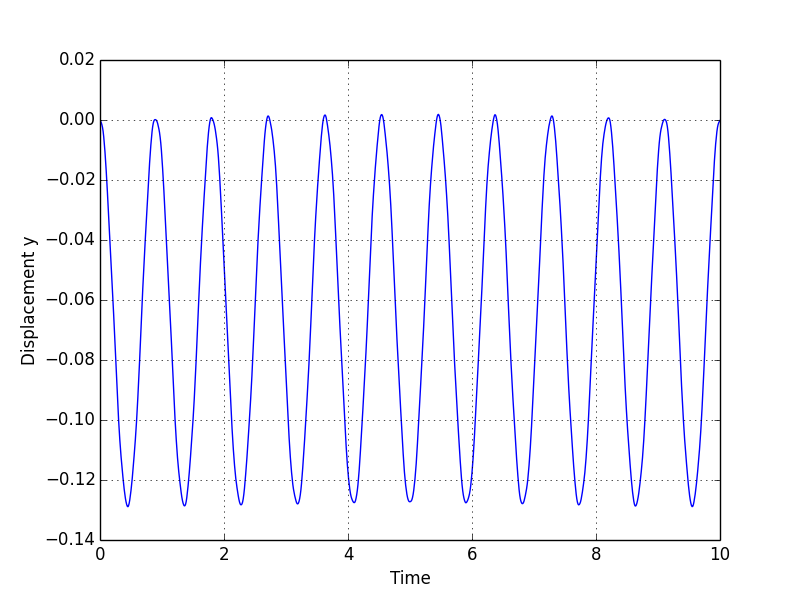
\includegraphics[width=0.75\linewidth]{./Verification_Validation//Hron_Turek/dis_y.png} 
    \caption{Displacement in x-direction} 
    \label{fig7:b} 
    \vspace{4ex}
  \end{subfigure} 
  \begin{subfigure}[b]{0.5\linewidth}
    \centering
    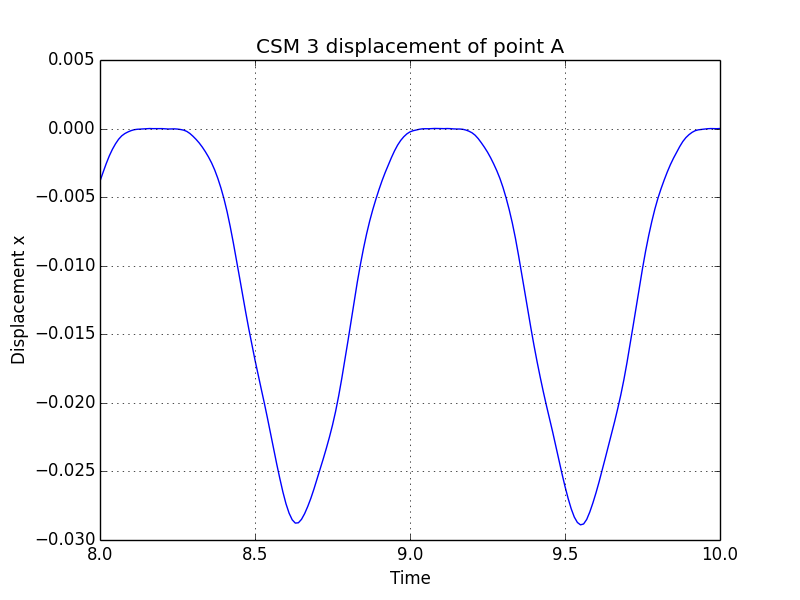
\includegraphics[width=0.75\linewidth]{./Verification_Validation//Hron_Turek/dis_x_short.png} 
    \caption{Displacement in x-direction} 
    \label{fig7:c} 
  \end{subfigure}%%
  \begin{subfigure}[b]{0.5\linewidth}
    \centering
    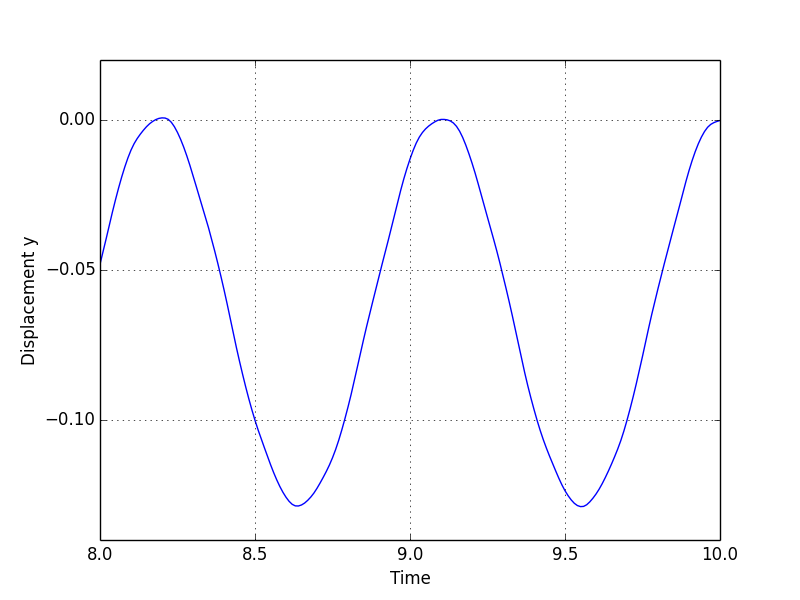
\includegraphics[width=0.75\linewidth]{./Verification_Validation/Hron_Turek/dis_y_short.png} 
    \caption{Displacement in x-direction} 
    \label{fig7:d} 
  \end{subfigure} 
  \caption{Displacement of point A}
  \label{fig7} 
\end{figure}


\subsection*{FSI test}
\begin{table}[ht]
\centering
\caption{FSI Parameters}
\label{my-label}
\begin{tabular}{|l|l|l|l|}
\hline
Parameters & FSI1 & FSI2 & FSI3 \\ \hline
$\rho_f[10^3 \frac{kg}{m^3}]$ & 1 & 1 & 1 \\ \hline
$\nu_f [10^{-3} \frac{m^2}{s}]$ & 1 & 1 & 1 \\ \hline
$u_0$ & 0.2 & 1 & 2 \\ \hline
Re = $\frac{U d}{\nu_f}$ & 20 & 100 & 200 \\ \hline
$\rho_s[10^3 \frac{kg}{m^3}]$ & 1 & 10 & 1 \\ \hline
$\nu_s$ & 0.4 & 0.4 & 0.4 \\ \hline
$\mu_s[10^6 \frac{m^2}{s}]$ & 0.5 & 0.5 & 2 \\ \hline
\end{tabular}
\end{table}
Results: 
\begin{table}[h]
\centering
\caption{FSI 1}
\label{my-label}
\begin{tabular}{|l|l|l|l|l|l|l|}
\hline
Cells & Dofs & ux of A $[x10^{-3}]$ & uy of A $[x10^{-3}]$ & Drag & Lift & Spaces \\ \hline
2698 & 7095 & 0.0234594 & 0.797218  & 14.4963 & 0.915801 & P1-P1-P1 stab= 0.01 \\ \hline
2698 & 23563 &0.0227418 &0.799314  &  14.1735 &0.761849 & P2-P2-P1 \\ \hline
10792 & 92992  &0.0227592 & 0.80795 & 14.1853 &  0.775063 &  P2-P2-P1 \\ \hline
43168 & 369448 & 00.227566 & 0.813184 & 14.2269 & 0.771071 & P2-P2-P1 \\ \hline
\textbf{ref} & \textbf{ref} & \textbf{0.0227} & \textbf{0.8209} & \textbf{14.295} & \textbf{0.7638} & \textbf{ref} \\ \hline
\end{tabular}
\end{table}



\newpage
OLD SHITZ FSI:
\begin{table}[h]
\centering
\caption{FSI 1}
\label{my-label}
\begin{tabular}{|l|l|l|l|l|l|l|}
\hline
Cells & Dofs & ux of A $[x10^{-3}]$ & uy of A $[x10^{-3}]$ & Drag & Lift & Spaces \\ \hline
2698 & 7095 & 0.0234594 & 0.797218  & 14.4963 & 0.915801 & P1-P1-P1 stab= 0.01 \\ \hline
2698 & 23563 & 0.02271 & 0.80288 & 14.1736 & 0.787891 & P2-P2-P1 \\ \hline
2698 & 23563 & 0.00581116 & 0.000000738678  & 12.07 & 0.02345 & P2-P2-P1 without weighting \\ \hline
10792 & 92992 & 0.0227341 & 0.808792 & 14.1855 & 0.801044 & P2-P2-P1 \\ \hline
43168 & 369448 & 0.227352 & 0.812595 & 14.227 & 0.797242 & P2-P2-P1 \\ \hline
\textbf{ref} & \textbf{ref} & \textbf{0.0227} & \textbf{0.8209} & \textbf{14.295} & \textbf{0.7638} & \textbf{ref} \\ \hline
\end{tabular}
\end{table}
%\newpage
\newpage
\section{Flexible tube}
This benchmark details fluids in flexible cylindrical tubes \cite{Greenshields2005}, which is relevant to practical problems as pressure surge in pipelines and blood flow in arteries. Specifically this deals with wave propagation due to pressure drop. Pressure will be added to one side of the cylinder producing a wave in which theoretical wave and flow speed can be calculated and compared to numerical findings.

\subsection{Problem definition}
\begin{center} 
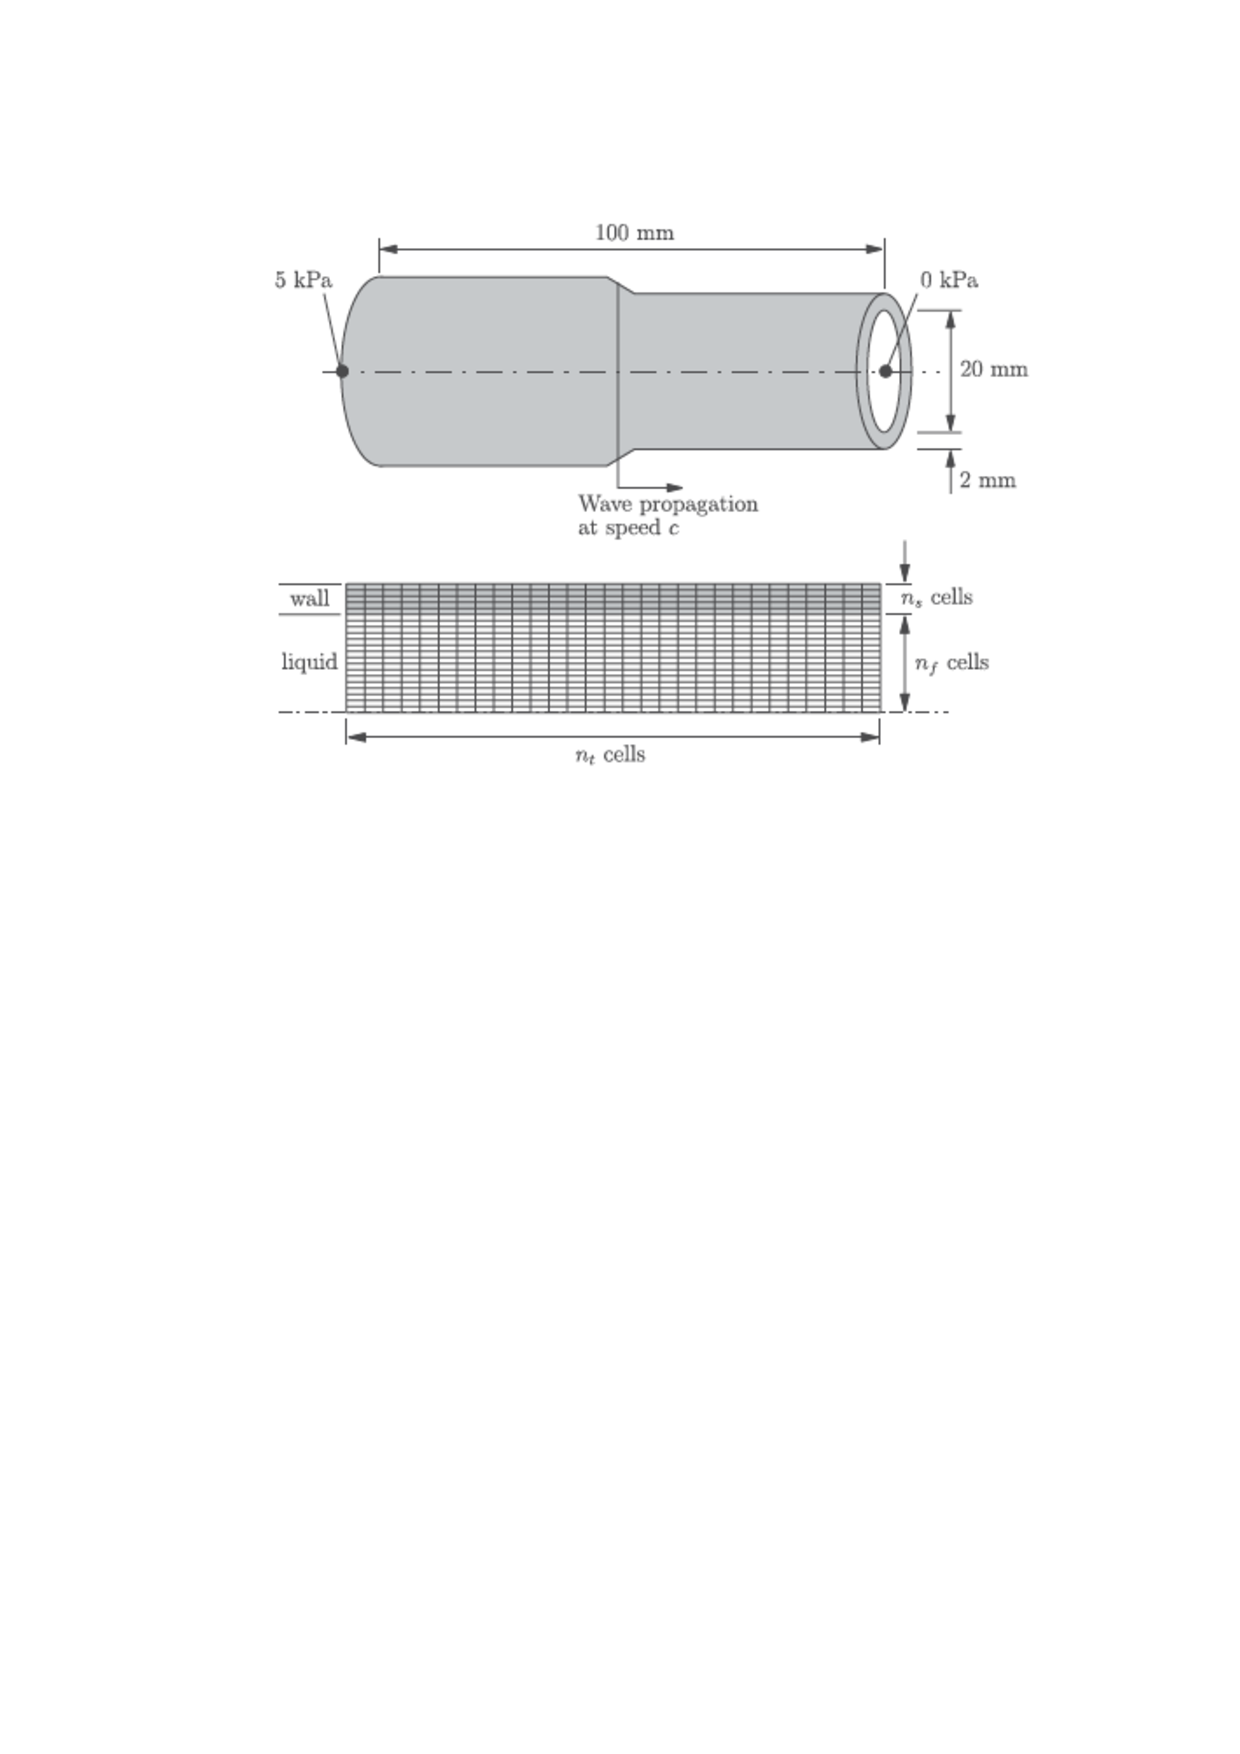
\includegraphics[scale=0.6,trim={0 15cm 0 10},clip]{./Verification_Validation/Flexible_tube/Pictures/definition.pdf}
\end{center}

The properties and geometry were selected for its representation of blood flow in a large artery. 

\subsection{Boundary conditions}


\subsection{Quanities for comparison}

\subsection{Results}
\begin{table}[h!]
\centering
\caption{My caption}
\label{my-label}
\begin{tabular}{|l|l|l|l|l|l|l|l|l|l|l|}
\hline
l {[}mm{]} & D {[}mm{]} & t {[}mm{]} & E {[}MPa{]} & $K_s [kPa] $ & $K_f [GPa]$ & $\nu_s $ & $\rho_s [\frac{kg}{m^3}]$ & $ \mu_s [kPa]  $ & $\rho_f []$ & $\mu_f [\frac{Ns}{m^2}]$ \\ \hline
100 & 20 & 2 & 1 & 833 & 2.2 & 0.3 & 1000 & 385 & 1000 & 0.0004 \\ \hline
\end{tabular}
\end{table}











